\documentclass{article}
%\usepackage{pgfplots}
%\usepackage{graphicx}
\usepackage{amsmath}
\usepackage{amsfonts}
\usepackage{mathtools}
\usepackage{pgfplots}
\usepackage{graphicx}
\usepackage{gensymb}
\usepackage[english]{babel}
\author{Yiqing(Alice) Guo}
\title{Assignment 2\\ \large CSCI-6390}

\begin{document}
\maketitle
\section{Part 1}
\subparagraph{}linear kernel project point:
\subparagraph{}[[-38292.4570163    2101.47455625]
\subparagraph{} [-38413.30362699   2978.28952548]
\subparagraph{} [-12268.52727985 -28345.6849681 ]
\subparagraph{} ..., 
\subparagraph{} [ 18548.88051646  -8111.42717031]
\subparagraph{} [ 17020.38035273 -15121.00127116]
\subparagraph{} [  3476.71591872  -7708.10369414]]
\subparagraph{} 5 dimensions are required to capture 95\% of the total variance
\subparagraph{}
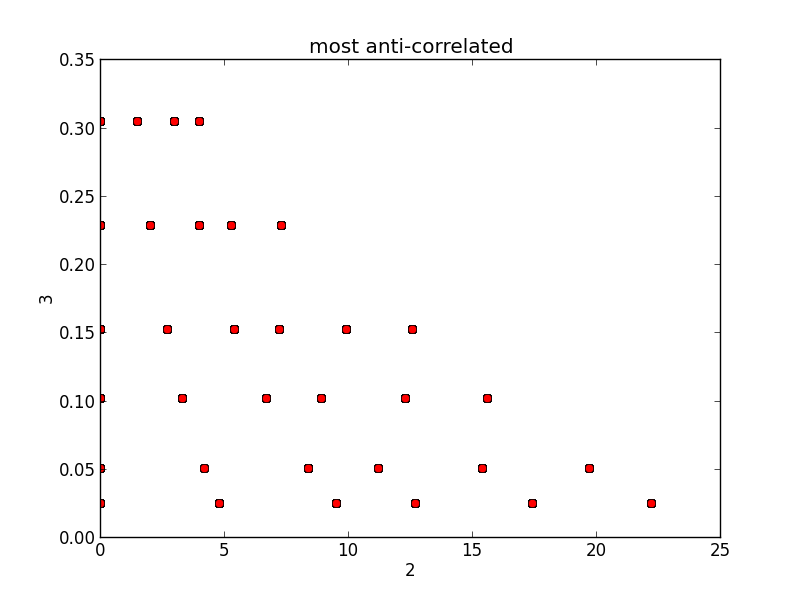
\includegraphics[scale=0.6]{figure_2}
\subparagraph{} PCA:
\subparagraph{}
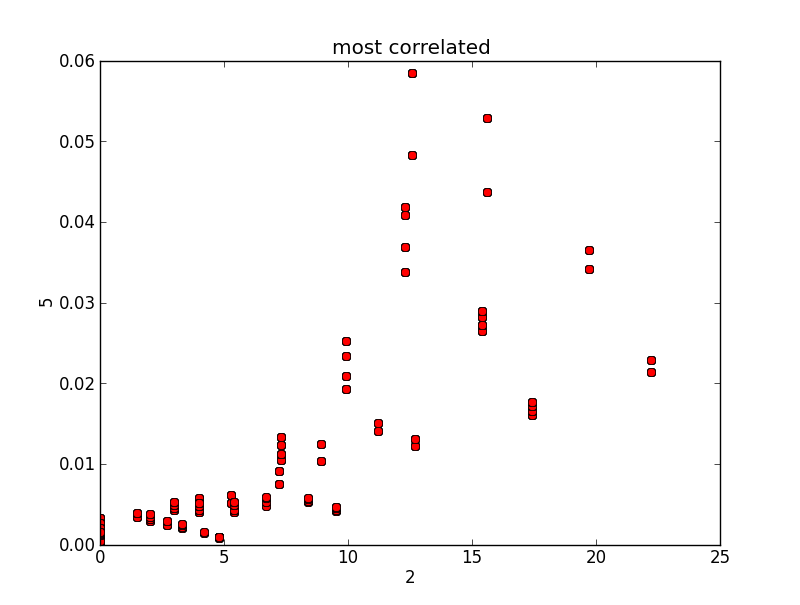
\includegraphics[scale=0.6]{figure_1}
\subparagraph{}Gaussian kernel(with $\sigma_2 = 2000$):
\subparagraph{}
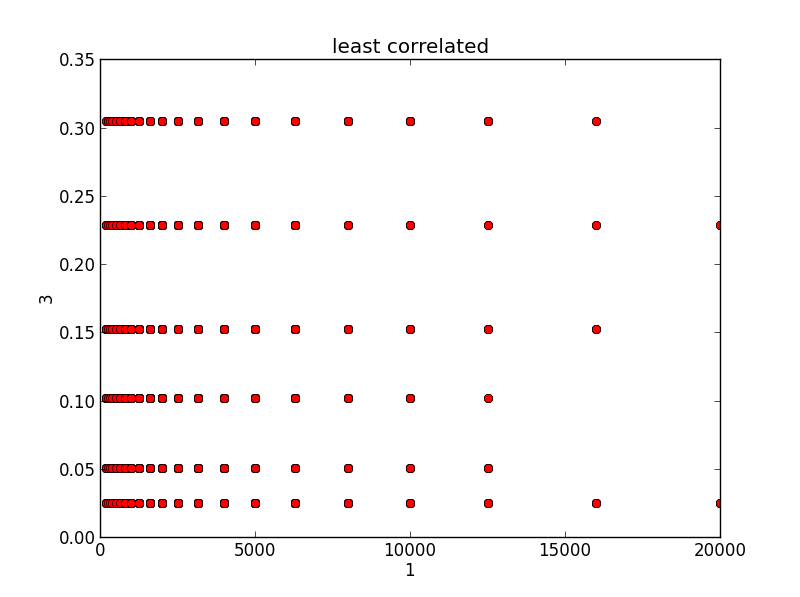
\includegraphics[scale=0.6]{figure_3}
\subparagraph{}How do the eigenvalues and the projection compare with that obtained via Kernel PCA with linear kernel?
\subparagraph{}The linear PCA and PCA have the same shape of plot bu different deriction and scale. 
\section{Part 2}
\subparagraph{}$N = 100, 000$, $d = 10$
\subparagraph{}Max: 180.0
\subparagraph{}Min: 0.0
\subparagraph{}Range value: 180.0
\subparagraph{}Mean: 89.9519671
\subparagraph{}Variance: 373.806371612
\subparagraph{}
\includegraphics[scale=0.6]{figure_1_part2}
\subparagraph{}$N = 100, 000$, $d = 100$
\subparagraph{}Max: 117.39
\subparagraph{}Min: 63.9
\subparagraph{}Range value: 53.49
\subparagraph{}Mean: 89.9812138
\subparagraph{}Variance: 33.2748129087
\subparagraph{}
\includegraphics[scale=0.6]{figure_2_part2}
\subparagraph{}$N = 100, 000$, $d = 1000$
\subparagraph{}Max: 97.47
\subparagraph{}Min: 82.53
\subparagraph{}Range value: 14.94
\subparagraph{}Mean: 90.0038613
\subparagraph{}Variance: 3.26839886336
\subparagraph{}
\includegraphics[scale=0.6]{figure_3_part2}
\subparagraph{}Extra Question:
\subparagraph{}As $d \to \infty$: we will have $\cos(\theta ) = \frac{v_1v_2}{d} = \frac{v_1v_2}{\infty}$
\subparagraph{}we will have $\cos(\theta ) = 0$ for $d \to \infty$ which is $90^{\circ}$, we have the EPMF trand as all points are close to the $90^{\circ}$ degree. we will certainly have mean = 90.
%\subparagraph{}Bonus Question:
%\subparagraph{}

\end{document}
